\chapter{Úvod}

Při vizualizaci různých systémů, kde máme nějaké objekty a spoje mezi nimi, jako jsou například sítě, grafy, apod., můžeme mít na zobrazení různé požadavky. Častým požadavkem je, aby se spoje nekřížili. Další možným požadavkem je, že objekty mají být zobrazeny \uv{blízko} sebe. Velmi podobným požadavkem se zabývá klastrová rovinnost, kde máme objekty seskupené do skupin nazývané klastry a požadavkem na vizualizaci je, aby každou skupinu bylo možno ohraničit do vymezeného regionu.

Problém existence rovinného klastrového nakreslení grafu (dále jen klastrová rovinnost) je jedním možným zobecněním klasické grafové rovinnosti pro případ, kdy kromě vrcholů a hran máme hierarchii skupin vrcholů. Skupinu vrcholů nazýváme klastrem. Pro klastrovou rovinnost není znám polynomiální algoritmus, a není známo, zda je tento problém NP-úplný. 

\begin{defn}
Mějme graf $G=(V,E)$. Pod \textit{klastrem} $C$ budeme uvažovat podmnožinu vrcholů  $C \subseteq V$. \\
\textit{Klastrovou hierarchií} jest množina klastrů, kde pro každé dva klastry $C_1$~a~$C_2$ platí následující
\begin{itemize}
\item buď $C_1 \cap C_2 = \emptyset$
\item nebo $C_1 \subset C_2$, případně nebo $C_2 \subset C_1$
\end{itemize}
\textit{Klastrový graf} je dvojice $(G,\mathcal C)$, kde $G$ je graf a $\mathcal C$ je klastrová hierarchie vrcholů G.
\end{defn}

Formálně se můžeme dívat na klastrovou hierarchii jako podmnožinu $\mathcal P (V)$. To může vést k tomu, že bychom si mohli myslet, že klastrů může být velmi mnoho vzhledem k velikosti původního grafu. V kapitole složitost ukážeme, že počet klastrů je lineární vzhledem k počtu vrcholů grafu $G$. V některých situacích se hodí předpokládat, že množina všech vrcholů vždy tvoří klastr a též jednotlivé vrcholy tvoří klastry. Například se tento předpoklad  hodí v důkazu o počtu klastrů.

\begin{defn}
Pod \textit{klastrovým nakreslením} rozumíme to, že vrcholy a hrany nakreslíme do roviny jako u rovinného nakreslení a navíc doplníme nakreslení klastrů.\\ 
\textit{Nakreslením klastru} $K$ v rovině je topologická kružnice $\gamma_K$. Vrcholy z $K$ leží ve vnitřku $\gamma_K$ a vrcholy nepatřící do $K$ leží vně $\gamma_K$. Hrany grafu smí protínat $\gamma_K$ nejvýše jedenkrát. Pro libovolné dva klastry se nesmí stát, že by se jejich nakreslení protínala.\\
Klastrový graf $(G,\mathcal C)$ je \textit{klastrově rovinný} pokud existuje nějaké jeho klastrové nakreslení.
\end{defn}

Omezení pro hrany v nakreslení klastru $K$ nám zaručuje, že hrany vedoucí mezi vrcholy klastru $K$ leží celé ve vnitřku $\gamma_K$.  Podobně hrany spojující vrcholy mimo $K$ musí ležet ve vnějšku $\gamma_K$. Definice nakreslení klastru nám zaručuje, že každá hrana křížící $\gamma_K$ spojuje vrchol z $K$ s vrcholem z $V \setminus K$.

Nyní můžeme úvest definici rozhodovacího problému klastrové rovinnosti. Klastrová rovinnost má dvě základní verze, a to nakreslená a nenakreslená verze.
\begin{defn}
V \textit{nenakreslené verze klastrové rovinnosti} máme rozhodnout, zda pro daný klastrový graf $(G, \mathcal C)$ existuje jeho klastrové nakreslení. Instanci nenakreslené verze klastrové rovinnosti budeme nazývat \textit{nenakreslený klastrový graf}. 
\\
U \textit{nakreslené verze klastrové rovinnosti} máme na vstupu trojici $(G, \mathcal C, \rho)$, kde $\rho$ je rovinné nakreslení $G$ a $(G, \mathcal C)$ je klastrový graf. Máme rozhodnout, zda lze $\rho$ rozšířit na klastrové nakreslení $(G, \mathcal C)$ dokreslením klastrů. Instanci nakreslené verze klastrové rovinnosti budeme nazývat \textit{nakreslený klastrový graf}.
\end{defn}

Nakreslená verze klastrové rovinnosti je už na pohled omezena silnější podmínkou a to nakreslením vstupního grafu. Pokud tedy nelze dokreslit klastry tak, abychom obdrželi klastrové nakreslení, pak klastrový graf stále může být klastrově rovinný (viz obrázek \ref{fig:obr1}).


\begin{figure}[H]
\centering
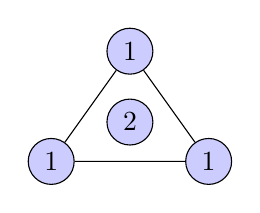
\begin{tikzpicture}[main_node/.style={circle,fill=blue!20,draw,minimum size=1em,inner sep=3pt]}]

    \node[main_node] (1) at (0,0) {1};
    \node[main_node] (2) at (-1, -1.4)  {1};
    \node[main_node] (3) at (1, -1.4) {1};
    \node[main_node] (4) at (0,-0.9) {2};

    \draw (1) -- (2) -- (3) -- (1);
\end{tikzpicture}
\caption{Čísla označují, do jakého klastru vrchol patří. Na první pohled je zřejmé, že není možné dokreslit klastr 1 tak, aby vrchol označený jako 2 nebyl ve vnitřku nakreslení klastru, ale je také zjevné, že příslušný klastrový graf je klastrově rovinný.}
\label{fig:obr1}
\end{figure}

Nyní definujeme několik pojmů, které jsou potřeba pro uvedení věty dávající kombinatorický pohled na problém klastrové rovinnosti. 

\begin{defn}
Mějme klastrový graf $(G,\mathcal C)$. Klastr $K$ je \textit{souvislý} pokud podgraf indukovaný na vrcholech klastru je souvislý. 
\end{defn}

\begin{defn}
Mějme klastrový graf $(G,\mathcal C)$, kde $G=(V,E)$. \textit{Saturátor} $S$ je podmnožina ${V \choose 2} \setminus E$ taková, že každý klastr je v $(G \cup S,\mathcal C)$ souvislý, kde $G \cup S = (V,E \cup S)$. \\
Mejme nakreslení grafu $G$, označme jej $\rho$. \textit{Nakreslený saturátor} $S$ je množina nakreslených hran takových, že nakreslení $\rho \cup S$ je rovinné nakreslení $G \cup S$ a v $G \cup S$ je každý klastr souvislý. 
\end{defn}

\begin{defn}
Mějme klastrový graf $(G,\mathcal C)$.V nakreslení $\rho$ grafu $G$ rozumíme \textit{dírou} kružnici $C$ v grafu $G$, jejíž vrcholy náleží klastru $K$ takovou, že v nakreslení $\rho$  je uvnitř nakreslení $C$ vrchol nepatřící do klastru $K$.
\end{defn}

Pokud má nakreslení $\rho$ grafu $G$ díru, tak jej nelze rozšířit na klastrové nakreslení, proto je zde uvádíme.
Větu o kombinatorickém pohledu na klastrovou rovinnost uvedeme zvlášť pro nakreslenou verzi a zvlášť pro nenakreslenou verzi.

\begin{theorem}[Di Battista, Frati \cite{DiBattistaFrati07}]
Nakreslený klastrový graf $(G,\mathcal C, \rho)$ je klastrově rovinný právě tehdy, když existuje nakreslený saturátor $S$ takový, že $(G \cup S,\mathcal C)$ nemá díru v $\rho$.
\end{theorem}

\begin{theorem}[Di Battista, Frati \cite{DiBattistaFrati07}]
Nenakreslený klastrový graf $(G,\mathcal C)$ je klastrově rovinný právě tehdy, když existuje saturátor $S$ takový, že $G \cup S$ má rovinné nakreslení, v němž není díra vzhledem k $(G \cup S,\mathcal C)$.
\end{theorem}